%--------------------------------Dependencies----------------------------------%
%   tikz                                                                       %
%       arrows.meta                                                            %
%-------------------------------Main Document----------------------------------%
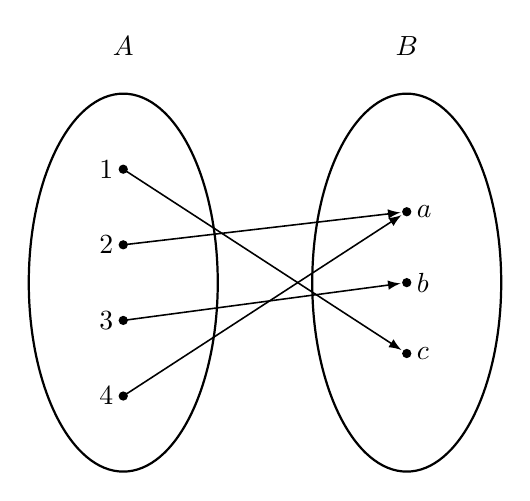
\begin{tikzpicture}[%
    >=latex,
    line width=0.2mm,
    line cap=round,
    scale=1.2
]
    % Coorindates.
    \coordinate (a) at ( 1.5,  0.75);
    \coordinate (b) at ( 1.5, -0.00);
    \coordinate (c) at ( 1.5, -0.75);
    \coordinate (1) at (-1.5,  1.20);
    \coordinate (2) at (-1.5,  0.40);
    \coordinate (3) at (-1.5, -0.40);
    \coordinate (4) at (-1.5, -1.20);
    \coordinate (A) at (-1.5,  2.50);
    \coordinate (B) at ( 1.5,  2.50);

    % Ellipses representing the sets A and B.
    \draw[thick] (-1.5, 0.0) ellipse (1 and 2);
    \draw[thick] ( 1.5, 0.0) ellipse (1 and 2);

    % Draw circles for the various points.
    \draw[fill=black] (a) circle (0.4mm);
    \draw[fill=black] (b) circle (0.4mm);
    \draw[fill=black] (c) circle (0.4mm);
    \draw[fill=black] (1) circle (0.4mm);
    \draw[fill=black] (2) circle (0.4mm);
    \draw[fill=black] (3) circle (0.4mm);
    \draw[fill=black] (4) circle (0.4mm);

    % Draw paths indicating mappings.
    \begin{scope}[->]
        \draw[shorten >=0.8mm] (1) to (c);
        \draw[shorten >=0.8mm] (2) to (a);
        \draw[shorten >=0.8mm] (3) to (b);
        \draw[shorten >=0.8mm] (4) to (a);
    \end{scope}

    % Labels.
    \node at (A)         {$A$};
    \node at (B)         {$B$};
    \node at (a) [right] {$a$};
    \node at (b) [right] {$b$};
    \node at (c) [right] {$c$};
    \node at (1) [left]  {$1$};
    \node at (2) [left]  {$2$};
    \node at (3) [left]  {$3$};
    \node at (4) [left]  {$4$};
\end{tikzpicture}